%% $RCSfile: proj_report_outline.tex,v $
%% $Revision: 1.3 $
%% $Date: 2016/06/10 03:41:54 $
%% $Author: kevin $

\documentclass[11pt
    , a4paper
    , twoside
    , openright
]{report}

\usepackage{float} % lets you have non-floating floats

\usepackage{url} % for typesetting urls

%
%  We don't want figures to float so we define
%
\newfloat{fig}{thp}{lof}[chapter]
\floatname{fig}{Figure}

%% These are standard LaTeX definitions for the document
%%
\title{The Title}
\author{Duy Nguyen}

%% This file can be used for creating a wide range of reports
%%  across various Schools
%%
%% Set up some things, mostly for the front page, for your specific document
%
% Current options are:
% [ecs|msor|sms]          Which school you are in.
%                         (msor option retained for reproducing old data)
% [bschonscomp|mcompsci]  Which degree you are doing
%                          You can also specify any other degree by name
%                          (see below)
% [font|image]            Use a font or an image for the VUW logo
%                          The font option will only work on ECS systems
%
\usepackage[font,ecs,mcompsci]{vuwproject}

\supervisors{Dr Alvin Valera \& Professor Winston Seah}
% You should specifiy your supervisor here with
%     \supervisor{Firstname Lastname}
% use \supervisors if there is more than one supervisor

\date{}

\begin{document}

% Make the page numbering roman, until after the contents, etc.
\frontmatter

%%%%%%%%%%%%%%%%%%%%%%%%%%%%%%%%%%%%%%%%%%%%%%%%%%%%%%%

%%%%%%%%%%%%%%%%%%%%%%%%%%%%%%%%%%%%%%%%%%%%%%%%%%%%%%%

\begin{abstract}

    % TODO: add abstract
    Load balancing in RPL using Machine learning

\end{abstract}

%%%%%%%%%%%%%%%%%%%%%%%%%%%%%%%%%%%%%%%%%%%%%%%%%%%%%%%

\maketitle

\chapter*{Acknowledgments}\label{C:ack} 
Thank you for Alvin and Winston for guiding me and helping me finish this project

\tableofcontents

% we want a list of the figures we defined
\listof{fig}{Figures}

%%%%%%%%%%%%%%%%%%%%%%%%%%%%%%%%%%%%%%%%%%%%%%%%%%%%%%%

\mainmatter

%%%%%%%%%%%%%%%%%%%%%%%%%%%%%%%%%%%%%%%%%%%%%%%%%%%%%%%

% TODO: introduction
% 1. RPL introduction
%    DODAG, DIO, DAO, DIS
%    Contiki-NG
%    CSMA and TSCH
%    COOJA and different mote types
% 2. Machine learning model
%    Regression model type
%    Data processing and optimisation
% 3. Decision Tree OF
%    Why?
%    Constrain of the model and OF
%    Experiment methodology
%    Data gathering: DIO update
%    Data processing and training process
%    Training the model and port to C
% 4. Evaluation
%    QoS: PDR, Latency, CPU usage
%    DIO overhead
%    Memory and ROM overhead
% 4. Limitation
%    Lack of real devices test
%    Overhead
% 5. Conclusion
% Literature review
% individual chapters included here
\chapter{Introduction}\label{C:intro}
Recent development in the Internet of Things (IoT) have driven a
rapid increase the number of devices connected to the Internet, with
growth continues to accelerate in many areas: health care,
construction, building.
These devices typically communicate wirelessly, exchanging data over
radio frequency links instead of relying on wired connections, which
allows flexible deployment across wide range of physical environments.
% TODO: may be cite the growth of IoT
However, many such deploymens invole large number of constrained
devices, which are bounded by low computational power, memory and energy
(battery), to cover large geographic areas.
% TODO: what is LLNs
Because the
underlying network technologies are limited in range, multi-hop
routing is often required. Such networks are categorised as
Low-power and Lossy Networks (LLN) as links in LLN are
susceptible to loss and frequent packet drops in addtion to contrains
on individual devices.

These limitations led the Internet Engineering Task Force (IETF),
which is an international organisation of network designers and
researcher, to form Routing over Low-power and Lossy networks (ROLL)
working group to investigate the routing solution for LLNs.
The working group first published RFC 5548 \cite{rfc5548}, RFC 5673
\cite{rfc5673}, RFC 5826 \cite{rfc5826}, RFC 5867 \cite{rfc5867} to
define the routing requirements for smart urban, industrial area,
home automation and building automation applications respectively.
From there, the ROLL working group had investigated the existing routing
protocols Open Shortest Path First (OSPF), Intermediate System to
Intermediate System (IS-IS), Ad hoc On-Demand Distance Vector (AODV),
and Optimized Link State Routing Protocol (OLSR), to which they found out that
they do not satisfy all of
the routing requirements. % TODO: include the reason why these protocols faile
This led to ROLL introducing a new routing protocol
designed specifically for LLNs called IPv6 based routing protocol for
low power and lossy networks (RPL), standardised in RFC 6550
\cite{alexanderRPLIPv6Routing2012}.

At its core, RPL constructs a Destination-Oriented Directed Acyclic
Graph (DODAG) to route packets from nodes toward a root, using
objective function (OF) to calculate path cost and select parents
during DODAG construction. Because of this, OFs determine how the
traffic is distributed across DODAG
% TODO: and directly affect the link quality and power usage.
% TODO: talk a bit more about this

% TODO: make this better
The protocol fell short when it comes to performing under high traffic as
load balancing was not considered in the design. Furthermore, the OFs
that ROLL propose only consider one metric, which might not be enough
to capture the inherent conditions of the network
Moreover, most of
the OFs are reactive in nature, meaning that would react after a
route has degraded, leading to decrease in network quality and reliability.

% TODO: make this better
In this project, we propose a new machine learning based OF that take
load balancing into account and predict the link quality to choose the parents

\section{Contribution}
% TODO: Add one more contribution
\begin{itemize}
    \item Contribute a new objective function based on machine
        learning which focuses on improving delivery ratio
    \item Investigate the feature importance of different metrics in
        determine the delivery ratio quality
\end{itemize}

\section{Organisation}
The rest of this report is structured as follow
\begin{itemize}
    \item Chapter \ref{C:Background} provides background information
        in relation to RPL and objective functions and related work
        in improving the objective functions
    \item Chapter \ref{C:ProposedOf} provides the motivation and overview
        the machine learning techniques and models used for our
        proposed objective function
    \item Chapter \ref{C:Experiments} shows the experiment and result
        from applying ML to OF
\end{itemize}

\chapter{Background and Related Work}\label{C:Background}

This chapter provides an overview of RPL and its load balancing objective functions in general. It then introduces the \ieeemac{} layer on which RPL operates, along with the energy model used for sensor devices. Finally, it describes the Contiki operating system and the COOJA simulator, which are used to simulate Contiki-based devices.

\section{Routing Protocol for Low-Power and Lossy Networks (RPL)}

RPL is an distance-oriented vector routing protocol that builds a
Destination-Oriented Directed Acyclic Graph (DODAG) over IEEE
802.15.4 PHY/MAC layers and 6LoWPAN (IPv6 over Low-Power
Wireless Personal Area Networks) \cite{alexanderRPLIPv6Routing2012}.
It is primarily designed for Wireless
Sensor Networks (WSNs),
where multipoint-to-point traffic toward one or more roots is the
predominant communication pattern.
Routes in RPL are optimised for traffic to or from one or more
roots in the topology, while maintaining reliable and energy
efficient data collection. To maintain reliable and energy-efficient
data collection, RPL is designed to adapt to changing
network conditions, allowing nodes to switch routes when route
degradation is detected.

\subsection{Destination-Oriented Directed Acyclic Graph (DODAG)}
RPL organises nodes under a DODAG, with the WSN's sink
node often serving as the root of DODAG. In a multi-sink deployment,
each sink node serves as the root of its own separate DODAG.
Within a DODAG, each node maintains a rank value, which is an estimation of the
distance between itself and the DODAG
root, and forms a directed edge toward a parent with a lower rank,
creating a herarchy network toward the root, as illustrated in
Figure~\ref{fig:dodag-example}. Thus within this
hierachy, the root always has the lowest rank.

% TODO: include how DODAG maintain loop free

A node's rank is computed by an objective function (OF), which
translates one or more metrics into rank, and the RPL
specification does not mandate a single OF for all applications.
Instead, RPL separates its core routing procedures --- packet
forwarding and DODAG maintenance --- from route optimisation, leaving
the choice of OF open to fit the diverse requirements of LLNs, such as
minimising energy consumption, reducing latency, or improving link
quality. This separation is what gives RPL the flexibility to support
such a wide range of applications, since a DODAG can be optimised for
whichever metric best suits its deployment.

\begin{fig}[H]
    \begin{center}
        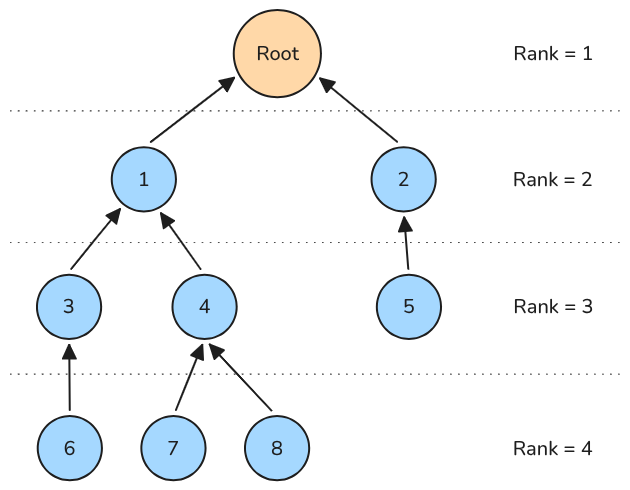
\includegraphics[width=0.6\textwidth]{assets/dodag.png}
        \caption{Example of a DODAG topology, showing nodes organised
        into a hierarchy rooted at the sink node.}
        \label{fig:dodag-example}
    \end{center}
\end{fig}

During DODAG construction, each node selects a parent from a pool of
candidate parents: neighbouring nodes that have already joined the
DODAG. The OF computes a candidate's resulting rank as
\[
    Rank(N) = Rank(P) + Rank\_Increase
\]
where $Rank(N)$ is the resulting rank of the node under consideration,
$Rank(P)$ is the rank already advertised by the candidate parent $P$,
and $Rank\_Increase$ is a positive value determined by the OF,
representing the cost of using $P$ as a parent. Because
$Rank\_Increase$ is always positive, a node's rank strictly increases
with each hop away from the root. The specific method used to compute
$Rank\_Increase$ and how parent is selected depends on the OF in use,
as discussed later in this chapter.

% There are four identifiers to define and maintain a topology in RPL shown in
% Table~\ref{tab:rpl-identifiers}.
% with RPLInstanceID and DODAGID used
% to identify a single DODAG in the network.
% % TODO: talk a bit more about why we have that many identifiers
%
% % TODO: talk about local and global repair
%
% % TODO: how to include identifier smoothly
% \begin{table}[h]
%     \caption{RPL DODAG identifiers} \label{tab:rpl-identifiers}
%     \begin{center}
%         \begin{tabular}{@{}p{0.25\linewidth}p{0.65\linewidth}@{}}
%             \hline
%             \textbf{Identifier} & \textbf{Description} \\
%             \hline
%             RPLInstanceID & The identifier of an RPL Instance, which may
%             span multiple DODAGs optimised for different applications. \\
%             DODAGID & The identifier of a specific DODAG within an RPL
%             Instance. \\
%             DODAG\-Version\-Number & The version number of a DODAG,
%             incremented by the root each time the DODAG is rebuilt to
%             distinguish between versions. \\
%             Rank & The estimated distance of a node from the DODAG
%             root; a node closer to the root has a lower rank. \\
%             \hline
%         \end{tabular}
%     \end{center}
% \end{table}

RPL introduces five types of control messages to form
and control DODAG, as specified in ICMPv6 via RFC 6550
\cite{alexanderRPLIPv6Routing2012}
\begin{itemize}
        % TODO: paraphrase this
    \item DODAG Information Object (DIO): carries information that
        allow nodes to discover a RPL instance, select parents and
        maintain the DODAG.
    \item DODAG Information Solicitation (DIS): a request message
        when a node want to join a DODAG
    \item Destination Advertisement Object (DAO): the node advertise
        itself to the root node, indicating that it has join DODAG
        and is reachable
    \item Destination Advertisement Object Acknowledgement (DAO-ACK):
        the acknowledgement of the root, confirming the downward path
        to the node
    \item CC: % TODO: what is this
\end{itemize}

To begin the DODAG forming process, the root node sends its DIO to
its neighbouring nodes, carrying RPL indentifiers and any
additional metrics required by the OF. Upon receiving DIO, a node
compares its rank with the advertised rank and filters out ranks that
are higher then its own to prevent loop formation, and then decides
whether to join the advertised DODAG or not.
In certain implementations, a node waits for several DIOs, building
the pool of candidate parents before deciding.
Afterward, the node computes the path cost of the
corresponding link for each candidate and determines the preferred
parent according the OF's policy.
Once a parent has been selected, the node broadcasts its own DIO to
advertise itself to its neighbours. This process is repated
outward through the network until every node has join the DODAG.
% TODO: may include diagram of how DIO transmission work

DIO is crucial in forming and maintaining DODAG, and DODAG requires
periodic DIOs to repair and update the conditions of the DODAG.
However, frequent DIO would be redudant in consistent network
conditions, thus RPL employs Trickle timer to regulate the emission of DIO.

% TODO: talk more about DAO
A node would send DAO message back to its parent or the root node to
establish downward communication.
In the DAO-ACK mode, a node wait
for the root node to send back DAO-ACK
before confirming that it is reachable and advertise DIO to surrounding nodes

% TODO: talk more about DIS
In addition for a node waiting to receive DIO to join DODAG, the node
can send DIS message to request DODAG information. When surrounding
nodes receive a DIS, it must unicast its DIO to that node, without
effecting the Trickle Timer policy. After receiving the unicasted
DIO, the node process the DIO as if it has receive a periodic DIO.

% TODO: write more about trickle timer
\subsection{Trickle Timer}
Trickle Timer is a scheduling algorithm based on consistency model.
The algorithm is structured in a way that would promptly send out DIO
during the formation process and would slow down when the DODAG has
been stablised.

adjusting the scheduling
regulates DIO transmission by adjusting the sending interval dynamically
based on the packets and network condition, ensuring timely DIO update
while reducing redundant message transmission \cite{rfc6206}.
The Trickle timer does this by evaluating the consistency of the
network message with its own state. However, the definition of
inconsistencies is left
for interpretation of the implementation. % TODO: give example of
% inconsistencies in RPL
In RPL specification, inconsistencies are defined as:
These inconsistencies$I$ include join new DODAG
version (e.g. new DODAGVersionNumber, new RPL instance, switching
parent), when % TODO: does switching parent reset DIO
nodes detect loop and additional inconsistencies according to the
implementation.
However, the specification leaves the implementation adds more
inconsistencies type when needed

When the network information is consistent, it
exponentially increases the transmission interval of DIO. However,
upon detecting inconsistencies, trickle timer reset its send interval
to boost DIO transmission to spread the latest information to the
rest of the DODAG.

Trickle Timer employs three configuration
parameters to determine the sending window of DIO: $I_{min}$, $I_{max}$ and $k$.
The maximum sending interval time is:
\[
    I_{max\_time} = I_{min} \times 2^{I_{max}}
\]

% TODO: give an example

Trickle timer set the initial sending interval $I$ in the range of
$[I_{min}, I_{max\_time}]$, usually the initial interval is set to $I = I_{min}$
% TODO: read more about trickle timer
The trickle timer will select a random time $t$ between $[I/2, I)$ as the
sending interval. When Trickle detects a consistent message, it will
increase the counter $c$,
At the time $t$, if the value of $c$ is less than the
redundancy constant $k$, the trickle transmits the message, otherwise
it would suppress the transmission.
After the interval $I$, Trickles double the time of the interval up
to $I_{max\_time}$ i.e. $I = max(I \times 2, I_{max\_time})$

Upon detecting inconsistent messages, The interval $I$ is reset to
$I_{min}$ to increase the DIO sending rate.

\begin{table}
    \caption{Trickle Timer Parameters}\label{tab:tricker_timer_params}
    \begin{center}
        \begin{tabular}[c]{@{}p{0.22\linewidth}p{0.10\linewidth}p{0.58\linewidth}@{}}
            \hline
            \textbf{Parameter} & \textbf{Symbol} & \textbf{Description} \\
            \hline
            Min interval length & $I_{min}$ & The minimum sending
            interval between two messages \\ % TODO: problably fix this
            Max interval length & $I_{max}$  & The maximum number of
            times that the sending interval can double \\
            DIO redundancy constant & $k$ & The number of consistent
            DIOs before suppresses its own DIO transmission \\
            \hline
        \end{tabular}
    \end{center}
\end{table}

\subsection{Communication Patterns}
% TODO: probably combine this with DIO transmission and DAO transmission
There are two types of communication patterns in RPL: upward route
and downward route
\subsubsection{Upward Route}
A node forwards packets toward the sink by relaying them to its
parent, which in turn relays them further up the tree until they reach the root.
Since a parent's rank is always lower than its child's and the root
rank is lowest, this process cannot get stuck in an endless cycle.

\subsubsection{Downward Route}
The downward are supported to P2MP and P2P route, in which the
destination is not the root node. In this pattern, the node sends DAO
to its preferred parent in a unicast manner

% TODO: study the storing mode more
In this pattern, the RPL specification defines two mode: storing mode
and non-storing mode. In storing mode, the downward routing tables
are included in each nodes
However, in non-storing mode, the downward routing tables are stored
only in the DODAG root. This means that P2P communication need to be
forwarded to the root node, where the root would then formulate the
routing path to the downward node.

% TODO: clarify this
The specification also opens option to specify DAO-ACK or not. A node
would only consider reachable only after it has received the DAO-ACK.

\subsection{OF0 and MRHOF}

Up to now, the IETF ROLL working group has standardised only two
objective functions: Objective Function Zero (OF0) \cite{rfc6552} and
Minimum Rank with Hysteresis Objective Function (MRHOF) \cite{rfc6719}.

% TODO: talk more about step of rank
OF0 was developed to be a simple objective function that utilise step
of rank, which is an intermediate computation based on link
properties of a certain neighbour.
, computing
$Rank\_increase$ as follow
\[
    Rank\_Increase = ( Rf \times Sp + Sr) \times Min\_Rank\_Increase
\]
where $Rf$ (Rank Factor) is a small positive integer used to scale
the step of rank; $Sp$ (Step of Rank) is an integer value
representing hop count in
abstract sense; and $Sr$ (Stretch of Rank) is used to inflate
$Rank\_Increase$ for
hysteresis preventing the OF from switching parents constantly.
We can select
OF0 parameters by
selecting $Rf = 1$, $Sp = 1$ and $Sr = 0$, which reduces
$Rank\_Increase$ to a simple fixed per-hop increment of 256. However,
The specification of OF0 strongly recommend computing step of rank
from Expected Transmission Count (ETX) to avoid blind hop count
measure, where it would select furthest
node to reduce the number of hops, leading to noisy and lossy link

OF0 can be regarded as implicitly using hop count as
routing metric. This mean that the traffic from OF0 follow the shortest path
to root without considering any load balancing requirement.
However, this also means that OF0 does not consider other link
qualities such as latency, energy residual in its calculation as well
as might choose worse off route but have the shortest hop count to root.
This led to the introduction a more sophisticated MRHOF.

In contrast, MRHOF propose multiple thresholds call hysteresis for
path cost and time
. In path cost threshold, unless the
potential node is better than the current parent by a threshold, it
will stick with the current parent. However, after the time
threshold, if that node is still better then the node will switch
parent. This would allows a more stabilised DODAG. Additionally,
MHROF allow choosing one from various metrics as the determing factor.

The default metric of MRHOF is Expected Transmission Count (ETX)
metric. The main goal of ETX is to select routes with high end-to-end
through put:
\[
    ETX = \frac{1}{D_t \times D_a}
\]
where $D_t$ is the probability that the receiving node receives the
packet and $D_a$ is the probability that the transmitting node
receives acknowledgement packet is successful. So ETX is the average
number of packets need to send and acknowledgement.
Since ETX is a floating point number while devices RPL operates on do
not generally support floating point arithmeic. The specifcation
indicates that 128 would be 1.0 ETX, improving the performace with
bitshift instead of expensive division.

% TODO: what word to describe route need less packets TX
In essense, using ETX as metrics focus on more transmission-efficient route.

There are two thresholds in MRHOF, rank threshold and time threshold.
The specification define $PARENT\_SWITCH\_THRESHOLD$ as the minimum
path cost improvement before deciding to switch.
There is time threshold, meaning that if a node consistently perform
better but not more than the ETX threshold, it still switch.

% TODO: include other metric container
The specification also open the choices of the routing metrics to energy,...
However, ETX is the more popular choice when it comes to MHROF.

Thanks to the flexibility of DIO header option.
% TODO: talk about the flexiblity of DIO

\section{Load Balancing in RPL}
Load balancing is an important issue in WSNs since devices are
expected to operate on battery for a long period of time. Some nodes
are used more frequently than others, especially the nodes near the
root, and exhaust their energy rapidly. These also includes when
there is an imbalance the traffic rate between node, where certain
nodes have higher data traffic than others e.g. videos or images,
thus selecting one parent would exhaust the possible routes to the parent node.

In this sense, load balancing is about distributing load from the
leaf to root node so that the node within the same hop share the
loads more evenly

These have to account for bursty traffic

% TODO: define what is load balancing
Despite that, RPL does not consider load balancing since it is
oriented to handling
low data traffic. Therefore, the network suffers in terms of latency,
delivery ratio and energy consumption under imbalance load senerios.

This is where OF0 and MRHOF fall short as they only consider one
metric: hop count and ETX. This does not capture the different
load of each node. Generally, ETX value does not change much when a
node experience heavy load \cite{kimQURPLQueueUtilization2015}

Another problem in load balancing is Thundering Herd problem, when a new node join the DODAG and advertise its existence. Since this node does not have any load, the neighbouring nodes would then choose this as their prefered parents, potentially overloading this node. While leaving their current parent free of load. When the current parent advertise itself, all the node would then switch, thus creating switch back and forth.
% TODO: insert image for thundering herd

% TODO: include other problems in load balancing as well


\section{Review of RPL Objective Functions Load Balancing}
\subsection{Related Work}
Various objective functions have been proposed, which can be
categorised into 4 groups: single metric, composite and context aware.

OF0 and MRHOF fit into single metric category.

% TODO: maybe include more OF0 and MRHOF evaluation
\cite{pradeskaPerformanceAnalysisObjective2016} evaluate  the
performance of OF0 and MRHOF in COOJA Contiki
Additionally, ... evaluates the performance of the standardised OFs
and find performance of OF0 degrade upon increasing load

In \cite{kimQURPLQueueUtilization2015}, the authors argues that most
of the losses are due to queue loss. Thus they used queue
utilisation metric in objective function, called QU-RPL to deal with
dropped packets due to queue overflow. Additionally, they also
modified the trickle timer to reset when a node experiences many
consecutive queue loss. With the changes, they achive lower queue
loss ratio and a more balance tree. However, only queue metrics are
taken into consideration, without mentioning latency.

A new objective function: OF-FL is presented in
\cite{gaddourOFFLQoSawareFuzzy2014}, which employs fuzzy logic with
four metrics with the aim of supporting various application requirements.
The authors used four metrics hop count, end to end delay, battery
level and ETX for categorise link quality. Each metric follows fuzzy
logic to indicate link quality from awful to excellent. The
simulation results show that OF-FL achieve higher PDR while
conserving more energy. However, the process of encoding each metrics into quality label is done manually and subject to the biases of the doers. % TODO: more about limitation in this

The authors in \cite{abreuEnergyawareRoutingBiomedical2014} propose an energy-aware objective function in RPL for healthcare monitor application. The nature of this problem means that the sensors is mobile, thus affecting the link quality % TODO: should I include this paper

The authors in \cite{taghizadehCLRPLContextAwareLoad2018} proposed Context-Aware and Load Balancing RPL (CLRPL). They introduced a new metric called Context-Aware Routing Metric (CARM), which considers queue utilisation and the percentage remaining power of a entire parents' chain from root the the node instead of the immediate parent. CARM would cnosider low-power parent but high-power overall route instead of rejecting it like energy of a single parent.
% TODO: include limitation of this 


Weighted Random Forward RPL (WRF-RPL) was propsoed in \cite{acevedoWRFRPLWeightedRandom2021}, which would select parents randomly based on weighted score % TODO: more about this

In recent, there has been many attempts to employ machine learning
into OFs. Despite that, most of the new application of ML in RPL
focues on reinforcement learning
with little focus on supervised learning

In \cite{duenassantosQRPLQLearningBasedRouting2024}, the authorse
puts Q-Learning to OF, award the model when a packet is trasmitted
successfully and penalise when choosing a link that lead to packet loss.
% TODO: include more reinforcement learning algo
% TODO: include the metrics name

There are three researches on applying supervised ML to RPL OF from a
research group. In RPL+ , the authors utilise Decision Tree to
perform feature importance evaluation with
six metrics ETX, channel utilisation, density, through put, queue
utilisation and MAC losses on data gathered hop by hop from
simulation \cite{duenassantosRPLImprovedParent2022}. They set
the $Rank\_Increase$ fixed to 1, which can be regarded as hop count,
and use the feature
importance as coefficients in linear equation and select parent with
the lowest score. Even though they improve the performance of PDR and
delay, the random forest model is only for feature importance
analysis and the training data only consider the success chance of
forwarded by one hop instead of the whole path. Additionally, having
fixed $Rank\_Increase$ means that the OF would select parents with
the shortest hop count.

In \cite{mezherGNBRPLGaussianNaive2023}, the research group train a
Naive Bayes classifier to predict the probability of a packet is sent
successfully or not on the same training feature as RPL+. This assume
that the distribution of the features fall into Gaussian distribution
In this paper, they train on more data and integrate the model into
the OF. However the evaluation lacks consideration for OF0.

Subsequently, the group proposed ML-RPL, using CatBoost model to
learn from eight metrics namely hop count, ETX, MAC losses, density,
channel utilisation, throughput, queu utilisation and RSSI
\cite{santosMLRPLMachineLearningBased2023}. Similar to previous
researches, this model predicts the predict the probability of
successfull one hop transmission. The evaluation of the results lack
energy or cpu util evaluation % TODO: more about limiation


% TODO: more discussion on the limitation of these papers

\section{IEEE 802.15.4 Protcol}

CSMA and TSCH

\section{Energy modeling}
Contiki-NG estimates energy consumption using a
software-based online mechanism proposed by
\cite{dunkelsSoftwarebasedOnlineEnergy2007}. It uses a linear
model in which each hardware component such as the CPU, the radio transmitter
and the radio receiver, draws a roughly constant current while it is active.

The total energy is then the sum of each component's active time
multiplied by its average current draw and the supply voltage:
\begin{equation}
    E = V \sum_{i} I_i \, t_i ,
\end{equation}
where $V$ is the supply voltage, $I_i$ is the average current draw of
component $i$, and $t_i$ is the time it spent active. Because the
estimation runs entirely in software, it needs no additional
measurement hardware and can easily be ported to different platforms.

Contiki-NG implements this model in its \emph{Energest} module, which
records how long each
component stays in each power state, measured in timer ticks.
Energest tracks give states. Three describe the MCU: active (CPU),
low power mode (LPM),
deep low power mode (DLPM). The other two describe the radio:
transmitting (TX) and receiving (RX). So the energy estimate in
Contiki-NG is calculated as follow. The time $t_x$ spent in each state is
obtained by dividing its tick count by the number of ticks per second
$t_x = \mathit{ticks}_x / \mathit{ENERGEST\_SECOND}$
And the energy consumed by a node is estimated as
\begin{equation}
    E = V \left( I_{\mathrm{CPU}}\, t_{\mathrm{CPU}}
        + I_{\mathrm{LPM}}\, t_{\mathrm{LPM}}
        + I_{\mathrm{DLPM}}\, t_{\mathrm{DLPM}}
        + I_{\mathrm{TX}}\, t_{\mathrm{TX}}
    + I_{\mathrm{RX}}\, t_{\mathrm{RX}} \right),
\end{equation}
where $V$ is the supply voltage, and $I_x$ and $t_x$ are the
average current
draw and the time spent in each state. In many cases where the energy
estimation is used to compare between
homogeneous nodes within the same network, V does not need to be
explicitly calculated to simplify the calculation.

The value of current drawn of each state is gathered from the
datasheet of the MCU and transceiver. Table~\ref{tab:current-draw}
shows the current drawn
of two platforms Z1 \cite{zolertia_z1} and Tmote Sky
\cite{moteiv_tmotesky} with transceiver CC2420 \cite{ti_cc2420}. The
current draw from datasheet should only be taken as a reference
point, which can vary a lot in different situation.

\begin{table}[htbp]
    \centering
    \caption{Average current draw per Energest state for the Zolertia
    Z1 and Tmote Sky platforms.}
    \label{tab:current-draw}
    \begin{tabular}{llcc}
        \hline
        \textbf{Component} & \textbf{State} & \textbf{Z1} &
        \textbf{Tmote Sky} \\
        \hline
        MCU   & Active (CPU)                 & 10\,mA       & 1.8\,mA \\
        & Low-power mode (LPM)         & 23\,$\mu$A   & 54\,$\mu$A   \\
        & Deep low-power mode (DLPM)   & 0\,$\mu$A    & 0\,$\mu$A    \\
        \hline
        Radio & Receive (RX)                 & 18.8\,mA     & 18.8\,mA     \\
        & Transmit (TX)                & 17.4\,mA     & 17.4\,mA     \\
        \hline
    \end{tabular}
\end{table}

% TODO: should I include this
% Time measurement is implemented using the on-chip timers
% of the MSP430. Since the on-chip timers work even when
% the microcontroller is in low-power mode, the time measure-
% ment is non-intrusive. We use the 32768 Hz clock divided
% by 8, producing 4096 clock ticks per second

From the table, radio power is much more significant than MCU power.
Since the removal of duty cycling layer in Contiki-NG in favor of
TSCH, the energy consumption in CSMA mode is dominated by radio
turning for the whole period.
However, TSCH is a much more complicated and memory heavy algorithm
for such old devices. Hence we opt for CSMA and use active CPU ticks
as intermediate value to measure the energy consumption relative to
other nodes in the network.

\section{Contiki-NG and COOJA Simulator}
\subsection{Contiki}
% TODO: cite ContikiOS
Contiki-NG is a lightweight operating system for resource-constrained
devices in WSNs and IoT.

which was built on the Contiki.

The Swedish Institute of Computer Science (SICS) released the first
version of Contiki in 2003 % TODO: cite this
Contiki was created by Adam Dunkels in 2002, which supports various
protocol for IoT devices
and have been support from various research instutitions
Later on, ContikiMAC was introduce as the sole duty cycle MAC layer for RPL.

% TODO: paraphrase this paragraph
However, recently a new Contiki cross-platform has been released on
Nov 2017 named Contiki-NG 4.0, which licensed under the 3-clause BSD
license. Contiki-NG concentrates on the Next-Generation IoT devices
such as ARM Cortex M3 and other 32-bit MCUs and on reliable and
secure standard protocols like IPv6/6LoWPAN, 6TiSCH, RPL, and CoAP
\cite{ContikiNG}.

In Contiki-NG, RPL implementation was rewritten as RPL-lite while the
original version of RPL in Contiki is kept as RPL-classic. RPL-lite
removes certain features RPL based on year of experience, keeping the
supports one single DAG at a time, one single “RPL instance”, and
only the non-storing mode of operation.

Addionally, ContikiMAC was removed in favor of TSCH implemetation,
thus making TSCH the default for duty cycle MAC implementation.

\subsection{COOJA Simulator for Contiki-NG}
The Cooja simulator is widely used among RPL OF researches % TODO:
% reference here

Cooja is an elastic Java-based simulator dedicated for WSNs based on
Contiki Operating System.
Cooja is capable of simulating different node types, including
simulated hardward (consisting of clock cycle and MCU) and software
based simulation (which skip the internal working of an MCU).

In this regard, Cooja is a tool for real hardware simulation.

depends on the mote type, provides three mote types out-of-the-box:
Sky, Z1 and Cooja where Sky and Z1 are emulated hardware for TelosB
and Zolertia Z1 and Cooja is the software simulation.
Table~\ref{tab:mote-specs} summarises the board specification.

% TODO: double checkthe MCU and Transceiver
\begin{table}[h]
    \caption{Supported mote hardware specifications in COOJA simulator}
    \label{tab:mote-specs}
    \begin{center}
        \begin{tabular}{lll}
            \hline
            \textbf{Specification} & \textbf{Zolertia Z1} & \textbf{TelosB} \\
            \hline
            Microcontroller        & MSP430F2617 (2nd gen)     & Texas
            Instruments MSP430 \\
            CPU                    & 16-bit RISC @ 16\,MHz     & 8\,MHz \\
            RAM                    & 8\,KB                     & 10\,KB \\
            Flash memory           & 92\,KB                    & 48\,KB \\
            Transceiver            & CC2420, IEEE 802.15.4     & Chipcon,
            IEEE 802.15.4 \\
            Frequency band         & 2.4\,GHz                  & 2.4\,GHz \\
            Data rate              & 250\,kbps                 & 250\,kbps \\
            \hline
        \end{tabular}
    \end{center}
\end{table}

Thus to maximise the computing power for machine learning model, Z1
is the most suitable mote for our need.

% TODO: paraphrase this
This platform is a virtual platform, used by the Cooja platform to
run Contiki-NG as ‘Cooja motes’. It compiles Contiki-NG as a native
process, and connects directly all hardware accesses to the Cooja
simulator. Unlike emulations, simulation with Cooja motes are not
perfectly time-accurate, but the timing is still good enough to run
the MAC layers CSMA and TSCH


\chapter{Machine Learning}\label{C:MachineLearning}
In this chapter, I will discuss about the machine learning models in IoT devices

\section{Regression Machine Learning Model}
The advance of machine learning has led the wide applications in IoT devices.

KNNR: works by comparing a node with the surrounding nodes to predict a value. In a sense, KNNR is considered a lazy model, in which it remembers all training data, thus result in a heavy model

Gaussian Process Regressor, similar to SVM. However, in \cite{}, the authors analyse GPR and conlcude that the memory requirement of GPR is $O(n^2)$ while the computation cost is $O(n^3)$, which is quite computational and memory expensive for constrained devices

Deep learning is recently a new adavnces and has achieve in terms of matching the complex patterns and data. However, due to the constrained environment of the working MCU which has several KB of RAM and ROM. I rule out this.

Random forest and Decision Tree operates on similar algorithm. In tree base algorithm, each value is split into left and right, following the path to reach the end. In Random Forest, multiple trees are used to prevent overfitting and provide better performance. However, in my experiments, the performance of random forest and decision tree are quite similar to each other. Thus I remove random forest from list of considered models as they are much heavier than decision tree.

\chapter{Experiments}\label{C:Experiments}

\section{Methodology}

The OFs are simulated in COOJA, using Z1 mote
Table ... list the running parameters for the experiment
\chapter{Performance Evaluation}\label{C:Evaluation}

\section{Topology generation}

In this section, we analyse the measurements of MLOF against OF0 and
MRHOF from result obtained from 120 simulations in COOJA simulator
using Z1 mote. Table~\ref{tab:sim-parameters} shows the training parameters

\begin{table}[h]
    \caption{Simulation parameters}
    \label{tab:sim-parameters}
    \begin{center}
        \begin{tabular}{ll}
            \hline
            \textbf{Parameter} & \textbf{Value} \\
            \hline
            Simulator                      & COOJA \\
            Mote type                      & Zolertia Z1 \\
            Simulation Time                & 1000\,s \\
            Number of Nodes                & 40, 60, 80 \\
            Sink Placement                 & Centralized \\
            Node Placement                 & Random \\
            Transmission rate              & 90\% \\
            Receiving rate                 & 90\% \\
            Topology                       & Random with seeds from 1-10 \\
            MAC Layer Protocol             & CSMA \\
            Data Rate                      & 250\,kbps \\
            Bandwidth                      & Up to 250\,kbps (refer to
            IEEE 802.15.4) \\
            Radio Range                    & 50\,m \\
            Interference Range             & 60\,m \\
            Packet Size                    & 64 bytes \\
            Routing Protocol               & MLOF, OF0 and MRHOF \\
            Packet per minute ($\lambda$) & 5, 10, 15 packets/minute\\
            Overloading client Packet per minute ($\lambda$) & 30 packets/minute\\
            Overloading client rate        & 5\% \\
            Confidence Level               & 95\% \\
            Statistical Test               & Paired t-test ($\alpha = 0.05$) \\
            \hline
        \end{tabular}
    \end{center}
\end{table}

\section{QoS Evaluation}
\subsection{Packet Delivery Performance}
PDR

\subsection{Latency}
Latency

\subsection{CPU Utilisation}
CPU util

\subsection{DODAG Stablity}
Parent switch

\section{Routing Overhead}
In the model, we added 7 fields, which increase the overhead

Memory analysis,

\section{Routing Topology}

\section{Effect of parameter $\alpha$}

\chapter{Conclusions}\label{C:con}
The conclusions are presented in this Chapter.

Limitation

\section{Future Work}


%%%%%%%%%%%%%%%%%%%%%%%%%%%%%%%%%%%%%%%%%%%%%%%%%%%%%%%

\backmatter

%%%%%%%%%%%%%%%%%%%%%%%%%%%%%%%%%%%%%%%%%%%%%%%%%%%%%%%

%\bibliographystyle{ieeetr}
\bibliographystyle{acm}
\bibliography{sample}

\end{document}
